% Asset ID: FAS2AlgorithmsOnGraphsTikZ-001
% Source: Supplied PDF/transcript Prim's algorithm worked example
% Related lesson section: Section 9 Visual Asset Integration
% Purpose: Show the weighted graph and selected minimal spanning tree edges.
\documentclass[tikz,border=8pt]{standalone}
\usepackage{xcolor}
\usepackage{tikz}
\usetikzlibrary{positioning,calc}
\definecolor{canvas}{HTML}{FAF9F6}
\definecolor{panel}{HTML}{FFFFF0}
\definecolor{line}{HTML}{E5E5EA}
\definecolor{accent}{HTML}{C5A059}
\definecolor{textcol}{HTML}{2C2C2E}
\definecolor{muted}{HTML}{9A9AA0}
\begin{document}
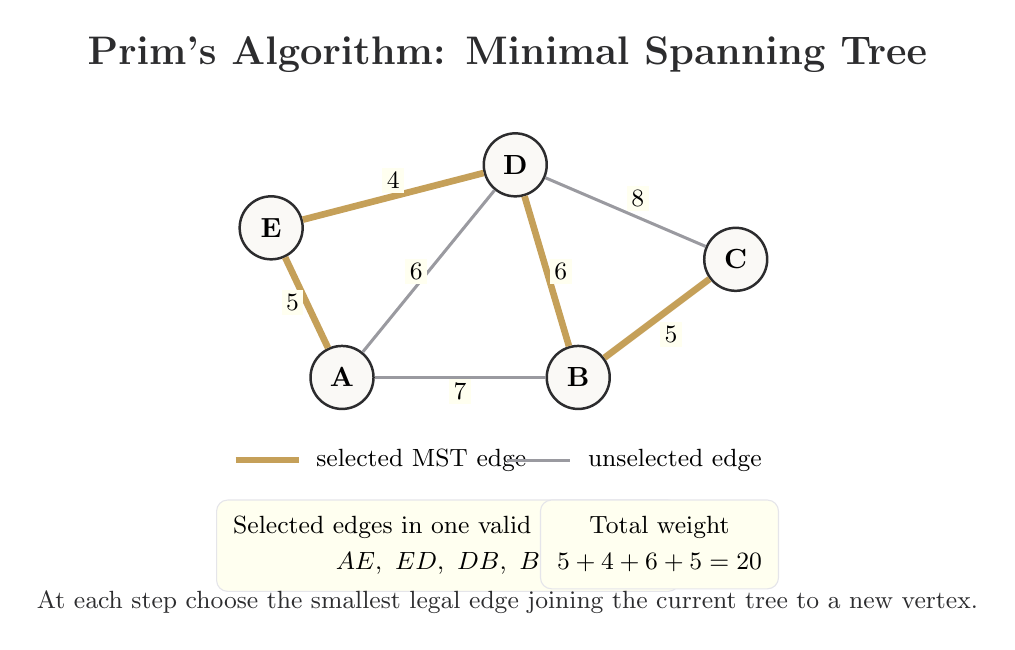
\begin{tikzpicture}[
    vertex/.style={circle,draw=textcol,fill=canvas,line width=0.9pt,minimum size=8mm,inner sep=0pt,font=\bfseries},
    unselected/.style={draw=muted,line width=1.1pt},
    selected/.style={draw=accent,line width=2.4pt},
    weight/.style={fill=panel,inner sep=1.6pt,font=\small},
    note/.style={draw=line,fill=panel,rounded corners=4pt,inner sep=6pt,align=center,font=\small}
]
\node[vertex] (A) at (0,0) {A};
\node[vertex] (E) at (-0.9,1.9) {E};
\node[vertex] (D) at (2.2,2.7) {D};
\node[vertex] (B) at (3.0,0) {B};
\node[vertex] (C) at (5.0,1.5) {C};
\draw[unselected] (A) -- node[weight,left] {$6$} (D);
\draw[unselected] (A) -- node[weight,below] {$7$} (B);
\draw[unselected] (D) -- node[weight,above right] {$8$} (C);
\draw[selected] (A) -- node[weight,left] {$5$} (E);
\draw[selected] (E) -- node[weight,above] {$4$} (D);
\draw[selected] (D) -- node[weight,right] {$6$} (B);
\draw[selected] (B) -- node[weight,below right] {$5$} (C);
\node[align=center,font=\Large\bfseries,text=textcol] at (2.1,4.1) {Prim's Algorithm: Minimal Spanning Tree};
\draw[selected] (-1.35,-1.05) -- (-0.55,-1.05); \node[anchor=west,font=\small] at (-0.45,-1.05) {selected MST edge};
\draw[unselected] (2.1,-1.05) -- (2.9,-1.05); \node[anchor=west,font=\small] at (3.0,-1.05) {unselected edge};
\node[note,anchor=north west] at (-1.6,-1.55) {Selected edges in one valid Prim order\\[2pt]$AE,\ ED,\ DB,\ BC$};
\node[note,anchor=north east] at (5.55,-1.55) {Total weight\\[2pt]$5+4+6+5=20$};
\node[align=center,font=\small,text=textcol] at (2.1,-2.85) {At each step choose the smallest legal edge joining the current tree to a new vertex.};
\end{tikzpicture}
\end{document}
